\documentclass{beamer}

\usetheme{Copenhagen}
\usepackage[utf8]{inputenc}
\usepackage{graphics}

% Slayt basliklarinda kullanilan font boyutu
\setbeamerfont{frametitle}{size=\normalsize}

\title{Geometric Constraints for Human Detection in Aerial Imagery}
\author{Vladimir Reilly, Berkan Solmaz, Mubarak Shah}
\date{2010}
\institute[CVL]{Computer Vision Lab, University of Central Florida, Orlando,
USA}

\begin{document}

\frame{\titlepage}

\section[İçindekiler]{}
\frame{\tableofcontents}

\begin{frame}
	\frametitle{Özet}

	\begin{itemize}
		\item UAV görüntülerde insanları algılamak
		\item hedef, çok az sayıda piksel barındırır
		\item Bu çalışmada görüntüye ek olarak \textbf{metadata} kullanıldı
		\item zemin normali ve insan gölgesinin yönelimi bellidir
		\item gölge yönelimini otomatik belirleyecek yöntem de önerildi
		\item buradaki yöntem \textbf{tek} kare temellidir
		\item wavelet öznitelik kombinasyonu ve SVM kullanıldı
		\item VIVID dataseti kullanılmıştır
	\end{itemize}
\end{frame}

\section{Giriş}

\begin{frame}
	\frametitle{UAV}

	\begin{block}{UAV}
		Unmanned Aerial Vehicle
	\end{block}

	\begin{itemize}
		\item gözetim (surveillance), askeri, güvenlik
		\item detection, tracking, classification ve event analysis
		\item yakın zamana ait havadan detecting-tracking ile alakalı
 		      cite{cheng06} ve cite{xiao08} çalışmalar insanı algılayamaz
		\item yerdeyken ki çekimlerden insan analiziyle ilgili tonlarca çalışma
		      yapılmıştır: cite{dalal05}, cite{felzenswalb08}, cite{leibe05},
			  cite{mikolajczyk04} ve cite{sabzmeydani07}
	\end{itemize}
\end{frame}

\begin{frame}
	\frametitle{yerden X gökten}

	\begin{itemize}
		\item \textbf{yerden} olanlarda insan $128x64$ gibi büyük boyutludur (ör. INRIA
			  dataseti)
		\item ve karşı cepheden görür
		\item \textbf{gökten} olanlarda insan $24x14$ gibi çok küçüktür ve
			  görünür parçası yoktur
		\item yerden olanlara uygulanan yöntemler geçersiz olur
		\item havai makinenin hareketi dolayısıyla yönelim açısından çok büyük
			  varyasyona sahiptir
		\item ayırt edici özellikler siliktir, bu yüzden false detection oranı
			  yüksektir
		\item "Person Tracking in UAV video" @ cite{xiao07} ve cite{miller07}
	\end{itemize}
\end{frame}

\begin{frame}
	\frametitle {İlgili Makaleler}

	\begin{itemize}
		\item cite{xiao07} ve cite{bose04}, hareket bilgisini kullandı
		\item hareket eden nesneler Histogram of oriented gradients
			  (\textbf{HOG}: cite{dalal05}) + SVM yardımıyla sınıflandı
		\item insan durağansa? gölge olduğunda? bloblar birbirine benzer takip
			  güçleşir
	\end{itemize}
\end{frame}

\begin{frame}
	\frametitle {İlgili Makaleler}

	cite{miller07}

	\begin{itemize}
		\item Harris corner özniteliğini kullanmıştır
		\item daha sonra OT-MATCH filtreden geçirilir
		\item insanı şekillendiren nokta sayısı çok fazladır
	\end{itemize}
\end{frame}

\begin{frame}
	\frametitle {Makalenin Yaklaşımı}

	\begin{itemize}
		\item UAV platformundan elde edilen metadata:
		\item yerin normali ki insanın yönelimini verir
		\item önce gölge bulunur (daha fazla alanı kaplıyor)
		\item burada insanın yüksekliği ve gölge uzunluğu kullanılarak
		\item insan adaylarından wavelet öznitelikleri çıkarılır: geometrik
			  kısıtlama yaklaşımı
		\item SVM ile insan veya değil şeklinde sınıflandırılır
	\end{itemize}
\end{frame}

\begin{frame}
	\frametitle{Üstünlükleri}

	\begin{itemize}
		\item motion detection gereksizdir
		\item güçlü gölgeler performansı etkilemez
	\end{itemize}
\end{frame}

\begin{frame}
	\frametitle{Metadata}

	\begin{itemize}
		\item metadata yoksa, statik görüntüden gölge bulucular kullanılabilir
		\item fakat standart gölge bulucular (cite{xu06}, cite{finlayson06})
			gerçek veri üzerindeki başarımı
		\textbf{kötüdür}.
	\end{itemize}
\end{frame}

\begin{frame}
	\frametitle{Metadata: gölge bulucu}

	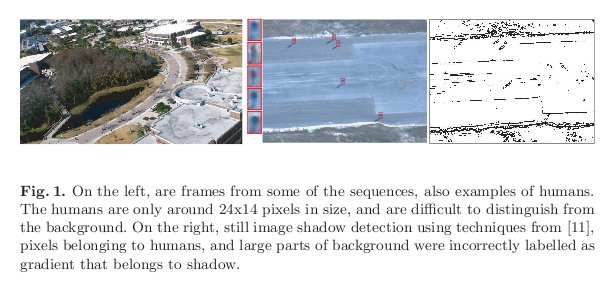
\includegraphics[width=1.0\textwidth]{img/fig1.jpg}

	Fig 1. databaseden bir kare, içerisinde insanlar var. İnsanlar yalnızca $24
	\times 14$ piksel boyutundadır, ve arkaplan ayırt etmek güçtür. cite{xu06}
	kullanılarak sabit görüntüde gölge algılama kullanıldığında, gövdeye ait
	pikseller ve arkaplanın büyük bir bölümü, gölgeye ait olarak yanlış
	etiketlenmiştir.
\end{frame}

\section{Yeryüzeyi Normali ve Gölge Kısıtlamaları}

\subsection{Metadata}

\begin{frame}
	\frametitle{Metadata}

	\begin{itemize}
		\item latitude, longitude, altitude parametrelerini içerir
		\item pitch, yaw, roll hesaplanabilir
		\item ayrıca kamera parametreleri: scan, elevation, twist (uçağa göre
			  değişimler), focal length, time
		\item dünyayla ilgili kısıtları belirler
	\end{itemize}
\end{frame}

\subsection{Dünya Kısıtlamaları}

\begin{frame}
	\frametitle{Dünya Kısıtlamaları}

	\begin{itemize}
		\item nesne algılama ve gözetim senaryolarında genelde gürültü olarak görülür
		\item havadan gözlem durumunda ise nesnenin kendisine ait bilginin
			  yetersizliğini tolere etmede kullanılır
		\item Kısıtlar şunlardır:
		\item kişi yeryüzeyine göre diktir
		\item kişinin gölgesi vardır
		\item kişinin yüksekliğiyle gölgesinin uzunluğu arasında geometrik
		ilişki vardır
	\end{itemize}
\end{frame}

\begin{frame}
	\frametitle{Sensör Modeli}

	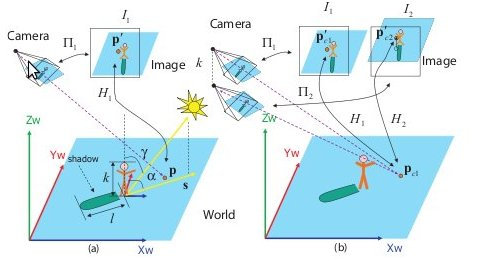
\includegraphics[width=0.8\textwidth]{img/fig2.jpg}

	Fig 2. \ref{fig:sensor-model}
\end{frame}

\begin{frame}
	\frametitle{Dünya Kısıtlamaları}

	\begin{itemize}
		\item latitude, longitude ve time belliyken (metadata)
		\item cite{reda03}'deki algoritma yardımıyla yer üzerindeki gözlemciyle
			güneşin göreceli konumunu elde edilir
		\item iki açı değeriyle tanımlanır: azimuth-$\alpha$, zenith-$\gamma$
		\item kişinin yüksekliği $k$ ise gölgesi $l = \frac{k}{tan(\gamma - 90)}$
		\item \label{eq:golge-olcekli}gölge uzunluğu azimuth-$\alpha$ açısıyla ölçeklenir:
			$S = <l	cos(\alpha), l sin(\alpha), 0>$
	\end{itemize}
\end{frame}

\subsection{Resim Kısıtlamaları}

\begin{frame}[allowframebreaks]
	\frametitle{Resim Kısıtlamaları}

	\begin{itemize}
		\item insan kısıtlamalarını devreye almadan önce dünya
			koordinatlarından $\rightarrow$ görütü koord. dönüştürelim
		\item burada metadata kullanılacak (ayrıntı için cite{hartley04})
		\item önce uçağın: latitude, longitude koordinatlarını dünya koord.
			dönüştür (bizde $X_w$=doğu, $Y_w$=kuzey)
		\item sensör modelini oluştur: herhangi bir piksel-$p'=(x_i, y_i)$'in
			dünya koordinatlarındaki karşılığı-$p=(X_w, Y_w, Z_w)$
		\item dönüşüm yapısı:
			\begin{equation}
				\Pi_1 = T^a_{Z_w} \times T^e_{X_w} \times T^n_{Y_w} \times
					R^y_{Z_w} \times R^p_{X_w} \times R^r_{Y_w} \times
					R^s_{Z_\alpha} \times R^e_{X_\alpha} \times R^t_{Y_\alpha}
					\label{eq:sensor-matrisi}
			\end{equation}
		\item burada $T^a_{Z_w}$, $T^e_{X_w}$ ve $T^n_{Y_w}$ uçak pozisyonunun
			dünya koordinatlarına dönüşümü için-altitude, east, north.
		\item $R^y_{Z_w}$, $R^p_{X_w}$ ve $R^r_{Y_w}$ uçağın dönme miktarı-yaw,
			pitch, roll
		\item $R^s_{Z_\alpha}$, $R^e_{X_\alpha}$ ve $R^t_{Y_\alpha}$ kameranın
			dönme miktarı-scan, elevation, tilt
	\end{itemize}
\end{frame}

\begin{frame}[allowframebreaks]
	\frametitle{Resim Kısıtlamaları: raytrace}

	\begin{itemize}
		\item 2d resim koordinatlarından-$p'=(x_i, y_i)$, 3d kamera koord.
			dönüştür- $\hat{p}'=(x_i, y_i, -f)$
		\item burada $f$ kameranın focal uznluğudur
		\item Eşitlik \ref{eq:sensor-matrisi} uygulanır ve yeryüzeyine raytrace
			yapılır
			\begin{equation}
				p = RayTrace(\Pi_1 \times \hat{p}')
				\label{eq:ray-trace}
			\end{equation}
		\item ray tracing, ortam hakkında geometrik bilgi talep eder: her bir
			piksel noktasındaki dünya yüksekliği gibi; bu ise DEM'den elde
			edilir.
		\item burada sahne planar olarak kabul edilmiş, ve yeryüzeyindeki
			noktalar-$Z_w=0$ yansıtılmıştır.
		\item herhangi bir piksel değeri-$p'=(x_i, y_i)$, raytracing ile
			yeryüzeyi noktasına-$p=(X_w,Y_w,0)$ dönüştürülür.
		\item sahnede yalnızca bir düzlem olduğundan, dört resim köşesine
			ihtiyaç duyuyoruz
		\item iki noktalar kümesi arasında Homography-$H_1$ hesaplanır:
			$p = H_1 \times p'$
		\item $H_1$, orijinal kareyi dikleştirecek (orthorectify) ve Kuzey
			Yönüyle hizalayacak
		\item Dikleştirme, resimden perspektif bozulmayı uzaklaştırır ve
			resimdeki dünya açısını ölçmeyi mümkün kılar
		\item dünya koordinatlarında tanımlı gölge vektörünü, resim
			koordinatlarına yansıtmada $H_1^{-1}$ kullanırız

			\begin{equation}
				S' = S \times H_1^{-1}
				\label{eq:diklestirme}
			\end{equation}
		\item buradaki $S$ (\ref{eq:golge-olcekli}) daha önceden verilmişti.

		\begin{itemize}
			\item kişinin yüksekliği $k$ ise, gölgesi
				$l = \frac{k}{tan(\gamma - 90)}$, burada $\gamma$-zenith açı değeri,
			\item gölge uzunluğu azimuth-$\alpha$ açısıyla ölçeklenir:
				$S = <l	cos(\alpha), l sin(\alpha), 0>$
		\end{itemize}
	\end{itemize}
\end{frame}

\begin{frame}[allowframebreaks]
	\frametitle{Sensör Modeli}

	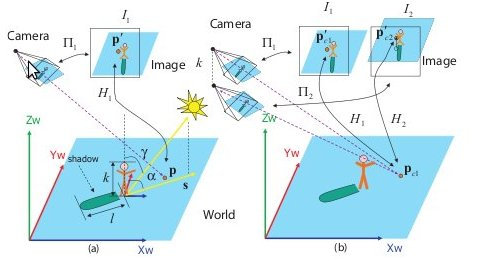
\includegraphics[width=0.9\textwidth]{img/fig2.jpg}\label{fig:sensor-model}

	\begin{scriptsize}
		Fig 2.
		Solda, sensör modeli $\Pi_1$, kamera koordinatlarından dünya koordinatlarına
		haritalar (görüntüyle kamera koordinat dönüşümü basitliğinden ötürü
		verilmedi). $X$, Doğu yönüne, $Y$, Kuzey yönüne, $Z$ dikey yöne işaret eder.
		$S$ vektörü, yeryüzeyi boyunca gözlemciden güneşe işaret eder. kuzey yönüyle
		güneş arasında kalan $\alpha$ azimuth açısıyla tanımlanır. $\gamma$ zentih
		açısı, dikey yönle güneş arasındaki açıdır. İnsan yüksekliği $k$ ve gölge
		uzunluğu $l$ olsun. Görüntü noktalarının dünya koordinatlarını bulmak için
		dünyada görüntü düzlemini yerleştirdik ve ona doğru raytrace ettik (görüntü
		düzleminden yeryüzeyi düzlemine yansıttık). Görüntü noktaları ve ona
		karşılık gelen dünya üzeri koordinatlar arasında $H_1$ homography si
		hesaplandı.

		Sağda, yeryüzeyi düzlem normalinin orijinal resimdeki yansımasının nasıl
		elde edileceğini gösterir. Daha düşük sensör modeli $\Pi_2$ kullanılarak,
		kamera koordinatlarındaki noktaları yeryüzeyi üzerindeki düzleme haritalayan
		diğer homography-$H_2$ elde edilir. $p_{c1}$ dünya noktasını $H_1$ ve $H_2$
		kullanarak haritalamak, $p_{c1}'$ ve $p_{c2}'$ görüntü noktalarını verir.
		$p_{c1}'$'den $p_{c2}'$'ye yönelen vektör, normal vektörün yansımasıdır.
	\end{scriptsize}
\end{frame}

\section{İnsan Algılama}
\subsection{Kısıtlamalı Arama}

\begin{frame}
	\frametitle{Başlangıç Adayları}

	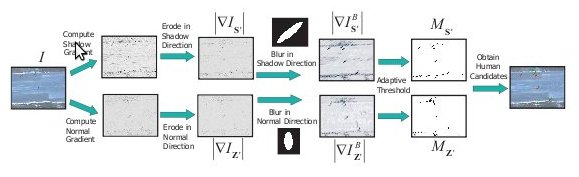
\includegraphics[width=0.95\textwidth]{img/fig3.jpg}\label{fig:baslangic-adaylari}

	Fig 3. başlangıç insan adayları kümesini elde etmek için uygulanan resim
	kısıtlamaları diagramını gösterir.

	\begin{itemize}
		\item metadatadan yönler (vücut ve gölge yönü) belli olduğuna göre
		\item ilgili yönlerde gradyan hesapla
	\end{itemize}
\end{frame}

\subsection{Nesne Gölge İlişkisinden Yararlanma}

\begin{frame}[allowframebreaks]
	\frametitle{Aday eleme}

	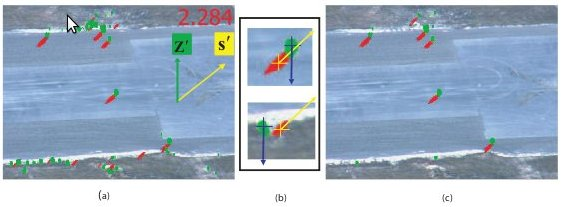
\includegraphics[width=0.8\textwidth]{img/fig4.jpg}\label{fig:aday-eleme}

	\begin{scriptsize}
	Fig 4. (a) gölge blob haritası $M_{S'}$ (kırmızı), normal blob haritası
	$M_{Z'}$ (yeşil). Resmin alt bölümünde false detection vardır. Sarı ok,
	yansıtılan günşe vektörü-$S'$ yansıtılan normal vektörü-$z'$ yeşil
	renklidir ve yansıtılan normal ve gölge uzunluğu arasındaki oran
	$2.284$'dir.

	(b) arındırılmış adayları gösteren bir örnekdir. Üsttekinde insan/gövde ve
	gölge blobları geçerli bir konfigürasyondadır ve hüzmeleri kesişmektedir, ve
	geçerli bir insan adayı olarak korunur. Alttakindeyse blobların
	konfigürasyonu geçersizdir, hüzmeler saçılmıştır (kesişim yok), ve insan
	adayları kümesinden çıkarılır.

	(c) her bir normal/gövde blobu onunla gölge blobunun ilişkilendirilmesi
	sonrasında korunmuş blob haritasını gösterir.

	\end{scriptsize}
\end{frame}

\subsection{Metada olmaksızın Kısıtlama}

\begin{frame}
	\frametitle{Metadata yokken}

	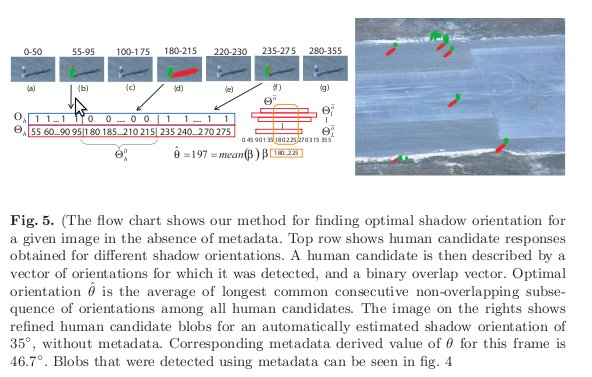
\includegraphics[width=0.95\textwidth]{img/fig5.jpg}\label{fig:optimal-shadow-orientation}

	\begin{scriptsize}
		Fig 5. Metada yokken, verilen resimdeki en uygun gölge yönelimini bulma
		yöntemi ayrıntılarını gösterir. Üst satır, farklı gölge yönlenmeleri için
		elde edilen insan adayı tepkilerini gösterir. Daha sonra, insan adayı,
		yönelim vektörüyle tanımlanır. Optimal yönelim-$\hat{\Theta}$, tüm insan
		adayları arasında en büyük ardışık örtüşmeyen yönelim dizisinin
		ortalamasıdır. Sağdaki resim, metadata olmaksızın, $35^o$ olarak otomatik
		tahmin edilmiş gölge yönelimi için korunmuş insan adayı bloblarını gösterir.
		Bu kare için metadata'dan türetilen $\Theta$ değeri, $46.7^o$'dir. Metadata
		kullanılarak algılanan bloblar ise Fig 4.'de verilmiştir
		(\ref{fig:aday-eleme}).
	\end{scriptsize}

	\begin{itemize}
		\item diğer gölge bulucular ve bizim yaklaşım denenebilir
	\end{itemize}
\end{frame}

\subsection{Nesne Adaylarını Sınıflama}

\begin{frame}
	\frametitle{Sınıflama}

	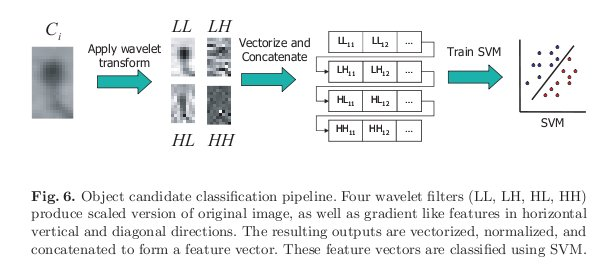
\includegraphics[width=0.95\textwidth]{img/fig6.jpg}\label{fig:classification}

	Fig 6. Nesne adaylarının sınıflandırılması. Dört wavelet filtresi (LL, LH,
	HL, HH) orijinal resmin ölçekle versiyonunu üretir. Elde edilen çıkışi
	vektöre dönüştürülür, normalize edilir ve öznitelik vektörünü biçimlendirmek
	üzere ardı ardına eklenir. Bu öznitelik vektörleri SVM yardımıyla
	sınıflandırılır.

	\begin{itemize}
		\item öznitelik kısmı iyileştirilebilir
		\item @ilke'ye verdiğim Türk bir hocanın kontur yaklaşımı kullanılabilir
	\end{itemize}
\end{frame}

\section{Sonuçlar}

\begin{frame}
	\frametitle{ROC: karşılaştırma}

	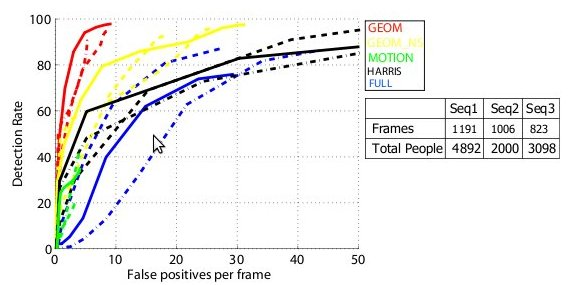
\includegraphics[width=0.8\textwidth]{img/fig7.jpg}\label{fig:ROC}

	\begin{scriptsize}
		Fig 7. ardışıllık 1 (çizgi-nokta), 2 (nokta) ve 3 (çizgi) için SVM güven ROC
		eğrisidir. Önerilen yöntem (gölge, nesne-gölge ilişki koruma ve merkezi
		konumlandırma temelli) kırmızı renkle gösterilmiştir. Sarı eğri, nesne-gölge
		ilişki koruma veya merkezi konumlandırma kullanılmadığında elde edilen
		eğridir. Standart tam kare algılayıcı (HOG) mavi renkle gösterilmiştir.
		Yeşil renk, cite{xiao07}'dekine benzer kayıtlanma, hareket, algılama ve
		izlemeyle elde edilen blob sınıflandırma sonuçlarıdır. Siyah eğri,
		cite{miller07}'in modifiye edilmiş gerçeklemesidir (Harris köşe bulucu
		kullanır).
	\end{scriptsize}
\end{frame}

\begin{frame}
	\frametitle{ROC: uzayı}

	\begin{columns}
		\column{0.5\textwidth}
			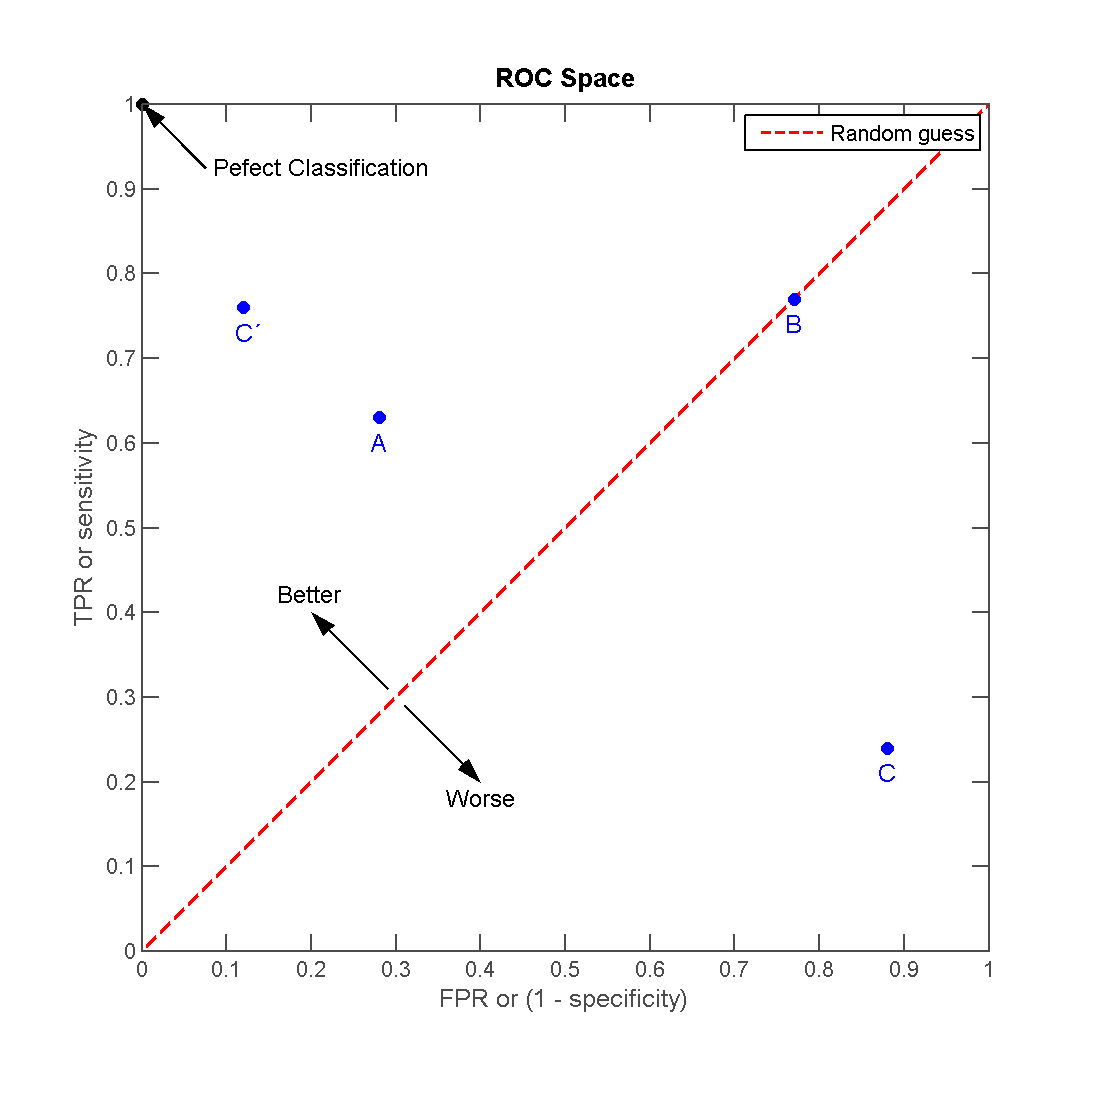
\includegraphics[height=0.8\textheight]{img/ROC_space.png}\label{fig:ROC-space}
		\column{0.5\textwidth}
			\begin{itemize}
				\item ROC (receiver operating characteristic) eğrisi,
					sensitivity (duyarlılık; True Pozitif Oranı) x False Pozitif
					Oranı (1 - specificity/özgüllük veya 1 - True Negatif
					Oranı); ayrım eşiğinin değişimiyle şekillenir.

				\item Bazen de ROC, TP/P (=TPR) X FP/N (=FPR).
			\end{itemize}
	\end{columns}
\end{frame}

\begin{frame}
	\frametitle{ROC: tanımlar}

	\begin{columns}
		\column{0.65\textwidth}
			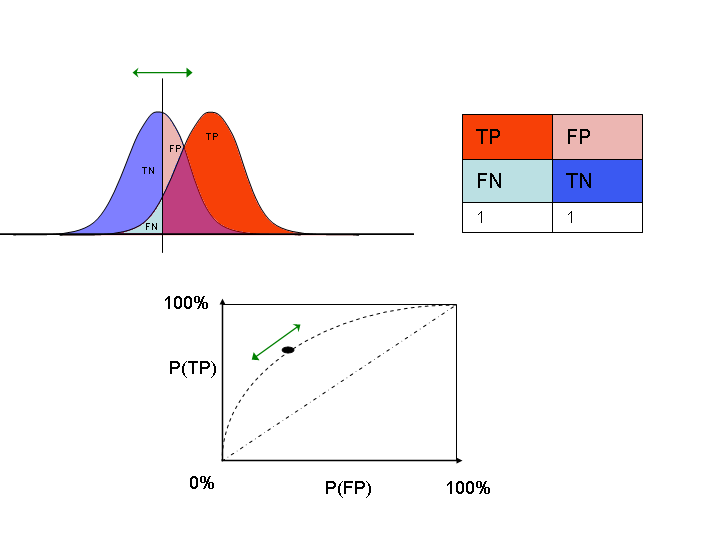
\includegraphics[width=1.0\textwidth]{img/ROC.png}\label{fig:ROC-def}
		\column{0.35\textwidth}
			\begin{itemize}
				\item TP / TN: Doğru sınıflandırma
				\item FP / FN: Hatalı sınıflandırma
				\item eksenler x:FP, y:TP; hatalı X doğru sınıflandırma
				\item mükemmel sınıflandırma sol-üst köşede olur
			\end{itemize}
	\end{columns}
\end{frame}

\begin{frame}
	\frametitle{Karşılaştırmalı Sonuçlar}

	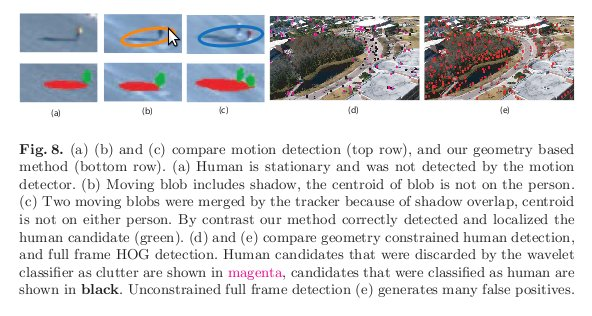
\includegraphics[width=0.8\textwidth]{img/fig8.jpg}\label{fig:compare}

	Fig 8.(a), (b) ve (c), hareket algılama (üst satır) ile önerilen yöntemi
	(alt satır) karşılaştırır. (a) İnsan, durağandır ve hareket algılayıcı
	arafından algılanamamıştır. (b) Hareketli blob, gölge içerir; blobun merkezi
	kişinin ki değildir. (c) iki hareketli blob birbirine girmiş; gölge
	örtüşmüş, merkez herhangi birine ait değil. Önerilen yöntem insan adaylarını
	doğru bir şekilde algıladı ve konumladı (yeşil). (d) ve (e) geometri
	kısıtlamalı insan algılama ve tam kare HOG algılayıcıyı karşılaştırır.
	Sınıflandırıcı yardımıyla adaylıktan çıkarılanlar mor, insan olarak
	işaretlenenler ise siyah olarak gösterilmiştir. Kısıtlamasız tam kare
	algılama (e) çok sayıda false pozitif üretmiştir.

\end{frame}

\section{Öneri}

\end{document}
